
\hypertarget{menu_marks}{}
\section{Marks}
\index{marks menu}

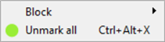
\includegraphics[scale=0.50]{./res/menu_marks.png}\\

\begin{scriptsize}
  \begin{tabularx}{\textwidth}{>{\hsize=0.3\hsize}X>{\hsize=0.7\hsize}X}\\
    \hline
    \textbf{Option} & \textbf{Description} \\
    \hline
    Block & \textit{\href{\#menu\_marks\_block}{See options ...}} \\
    Unmark all & Unmarks all marks of the current file \\
    \hline
  \end{tabularx}
\end{scriptsize}


\hypertarget{menu_marks_block}{}
\subsection{Block}
\index{marks menu!block}

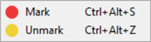
\includegraphics[scale=0.50]{./res/menu_marks_block.png}\\

\begin{scriptsize}
  \begin{tabularx}{\textwidth}{>{\hsize=0.2\hsize}X>{\hsize=0.8\hsize}X}\\
    \hline
    \textbf{Option} & \textbf{Description} \\
    \hline
    Mark & Marks selected block: \texttt{0 to begin} and \texttt{1 to end} \\
    Unmark & Unmarks any previous marked block. It is not necessary to select the marked block \\
    \hline
  \end{tabularx}
\end{scriptsize}
